\section{TOKIO Architecture \& Implementation} \label{sec:architecture}

\begin{figure}
    \centering
    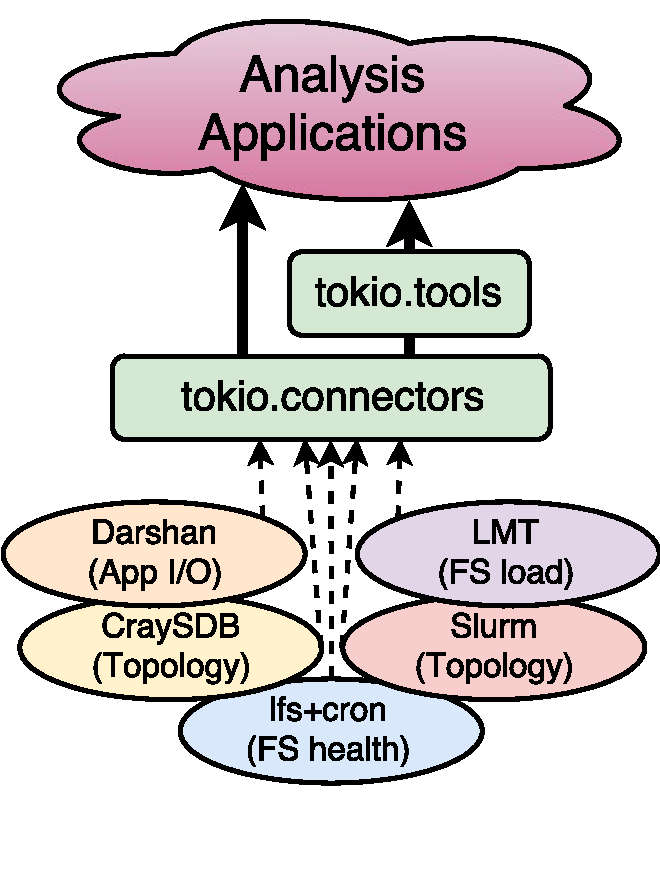
\includegraphics[width=0.7\columnwidth]{tokio-architecture-v3}
    \vspace{-.3in}
    \caption{TOKIO Architecture.  \texttt{tokio.connectors} take input from component-level monitoring tools in their native output formats and expose that data to upstream analysis in standard data formats such as key-value pairs, Pandas dataframes, and NumPy arrays. \texttt{tokio.tools} provide indices, site-specific data placement information, and enhanced usability.}
    \label{fig:tokio-architecture}
    \vspace{-.2in}
\end{figure}

To meet the design criteria outlined in Section \ref{sec:intro}, the TOKIO framework is comprised of four layers as shown in Figure \ref{fig:tokio-architecture}.
Each layer is then composed of modules which are largely independent of each other to allow TOKIO to integrate with whatever selection of tools a given HPC center has running in production.
That said, certain tools are \emph{de facto} standards for I/O performance analysis, and those tools will be highlighted in the following architectural description as examples of how TOKIO enables holistic analysis.

\subsection{Component-level monitoring tools} \label{sec:architecture/components}

Following design criterion \#\ref{design:existingtools}, TOKIO builds upon whatever monitoring and profiling tools are already in production at an HPC facility.
Although the tools and infrastructure supporting them exist outside of the scope of TOKIO, we identify several broad categories of metrics that are relevant to understanding I/O performance.

\subsubsection{Application behavior} \label{sec:architecture/components/application}

The I/O patterns that a program issues can affect performance dramatically regardless of the underlying storage system.
This behavior can be automatically profiled using tools like Darshan~{Carns2009}, which is a link-time library that transparently records concise, bounded statistics about an application's I/O behavior.  
It is commonly included with all compiled applications at CUG member sites including NERSC, ALCF, NCSA, and KAUST~\cite{Lockwood2017,Luu:2015:HPDC,Hadri2015,White2017}.
Complementary information from client-side monitoring  such as the collection of file system client metric collection enabled by RUR~\cite{Butler2014} also falls in this category.

In all cases, though, understanding application behavior can capture information about client-side caching and intra-node or intra-application contention~\cite{Lofstead2010} that may not be quantifiable from other parts of the I/O subsystem.
In addition, the sensitivity of application performance to jitter caused by ongoing performance monitoring on compute nodes results in application behavior data being discrete in nature.

\subsubsection{Storage system traffic} \label{sec:architecture/components/fs}

The servers that serve and store file data and metadata are inherently shared by all users of an HPC system, and as a result, are intuitively susceptible to resource contention from competing jobs.
It follows that monitoring the traffic and load on each storage system server is a valuable tool for identifying contention-related issues that may be beyond the visibility or control of individual users and their jobs.

Just as there are a variety of storage system implementations, there are a variety of implementation-specific tools for collecting these data.
On Cray ClusterStor systems, Lustre Monitoring Tools (LMT) have historically collected this data~\cite{Keopp2014}, and Cray's newer Caribou and Seastream infrastructure is being positioned as the preferred alternative for the future~\cite{Flaskerud2017}.
File system-specific tools for Cray DataWarp systems do not yet exist, but NERSC has demonstrated that collectd and ElasticSearch can collect and store device-level load data to similar ends~\cite{Whitney2016}.
Unlike application behavior data, collecting storage system traffic at high frequency results in very low perceptible jitter; as a result, it is commonly recorded as time series data with an ideal sampling rate of under ${^1 / _{60} \textup{ Hz}}$~\cite{Madireddy2017}.

\subsubsection{Storage system health}  \label{sec:architecture/components/fshealth}

There are many circumstances in which a component of a storage system is known to be in an available but degraded state of performance as a result of a temporary failure or condition.
Conditions such as storage device failovers (where a server may have to take on the load of a failed partner server) or RAID rebuilds (where device bandwidth is being consumed by reconstruction of data from parity) can introduce significant long-tail performance losses to files that are striped across those degraded devices.

As with storage system traffic data, storage system health data is often monitored using implementation-specific tools that understand architecture-specific failures that degrade performance.
In the case of Lustre, the \texttt{lctl dl -t} command is sufficient to identify failed-over OSTs, while \texttt{lfs df} provides information that implicates performance loss due to high file system fullness.
DataWarp can be monitored on a per-device basis using standard tools such as \texttt{smartctl} or vendor-specific tools such as the Intel SSD Data Center Tool~\cite{isdct}.

\subsubsection{Job topology} \label{sec:architecture/components/topology}

The effects of locality on I/O performance within high-diameter networks have been well documented~\cite{Vishwanath2011,Bui2014,Dillow2011}, and modern high-radix topologies continue to be susceptible to topology-induced performance variation~\cite{Mubarak2017}.
Obtaining the topological mapping of a given job's compute nodes across a given network fabric requires several different tools that combine job-node mappings from the system resource manager with the node-coordinate mapping from the system component which tracks global system state.

In practice, both of these tool sets are highly system-specific; the job-node mappings may be provided by a resource manager such as Slurm~\cite{Jacobsen2016} or ALPS~\cite{Karo2006}, and node-topology mappings are provided by the Cray Service Database.
Fortunately, the relationship between nodes and topological coordinates in the fabric is a relatively static mapping, and it can be aggressively cached so long as that cache is expired any time the fabric topology is altered.

\subsubsection{Network traffic} \label{sec:architecture/components/network}

The networks over which I/O transits, including both the high-speed network and the back-end storage fabric, are shared resources and therefore susceptible to contention from other workloads.
Unlike the storage system traffic data, though, network traffic loads tend to be very complex since they are a function of loads at both compute and storage server endpoints as well as incidental traffic being routed over the same links.

On Cray systems, the Gemini Counter Performance Daemon~\cite{Pedretti2013,Brandt2016} or AriesNCL~\cite{ariesncl} can be used to collect the performance counters available on Aries routers.
In practice, the complexity and scale of these network traffic data make them challenging to collect effectively.
LDMS~\cite{Agelastos2014ldms} has emerged as a scalable infrastructure for collecting these data system-wide, while PAPI has been demonstrated to collect these data on a per-job basis~\cite{Groves2017}.

\subsection{TOKIO connectors} \label{sec:architecture/connectors}

The foundational layer of TOKIO are \emph{connectors}, which are independent, modular components that provide an interface between the individual component-level tools described above and the higher-level TOKIO layers described later.
Each connector understands the API of the component-level tool with which it interfaces


In the pytokio implementation of TOKIO, connectors are classes that expose each component-level tool's data as dictionaries, dataframes, and arrays.

pytokio provides connectors for the following tools either available as community-supported open-source tools or pre-installed on Cray systems:

\begin{itemize}
\item \textbf{Cray SDB} for node topology
\item \textbf{Slurm} for job ID and node list mappings
\item \textbf{Darshan} for application-level I/O profiling
\item \textbf{Lustre} \texttt{lfs} and \texttt{lctl} for file system health
\item \textbf{LMT} for server-side Lustre loads via the ClusterStor Lustre monitoring tool~\cite{Keopp2014}
\end{itemize}

\subsection{TOKIO tools} \label{sec:architecture/tools}

provide convenience functions and wrappers around TOKIO connectors.  For example, TOKIO provides a \texttt{topology} tool which converts a user job ID into a job radius by converting the job ID into a node list using the Slurm connector, and then the node list into topological coordinates using the Cray SDB connector.

\subsection{Analysis applications} \label{sec:architecture/analysis}

perform statistical, analytical, and visual performance analyses by using TOKIO connectors and tools to combine data from multiple components.